\documentclass[12pt]{tcc}
\usepackage[brazil]{babel} 
\usepackage[T1]{fontenc}
%\usepackage[brazilian,hyperpageref]{backref}
\usepackage[hidelinks]{hyperref}
\usepackage[pt-BR]{datetime2}
\DTMlangsetup{showdayofmonth=false}
\usepackage[portuguese,ruled,linesnumbered,algochapter,titlenumbered]{algorithm2e}
\usepackage{listings}
\usepackage{xcolor}

% Define TypeScript language style
\lstdefinelanguage{TypeScript}{
    keywords=[1]{import, from, export, class, extends, private, void, constructor, super, this, async, await, for, of, let, in, return, any, console, log},
    keywordstyle=[1]\color{blue},
    keywords=[2]{Task, CompositeTask},
    keywordstyle=[2]\color{purple},
    keywords=[3]{forEach},
    keywordstyle=[3]\color{orange},
    ndkeywords={true, false, catch, function, null, undefined},
    ndkeywordstyle=\color{darkgray},
    identifierstyle=\color{black},
    sensitive=false,
    comment=[l]{//},
    morecomment=[s]{/*}{*/},
    commentstyle=\color{green}\ttfamily,
    stringstyle=\color{red}\ttfamily,
    morestring=[b]',
    morestring=[b]"
}


% As figuras ficam armazenadas na pasta figuras
\graphicspath{{./figures/}}

% Informações do trabalho
\newcommand\dtitle{Framework para Análise de Desempenho de Consultas Web}
\newcommand\dauthor{Filipe Shanom Glathardt de Azeredo Xavier\\Matheus dos Santos Moura\\Radhanama Dasa de Maria Moraes Mesiano}
\newcommand\dadvisor{Renato Campos Mauro}

% Definição de acronimos
\newacro{TCC}{Trabalho de Conclusão de Curso}
\newacro{QoS}{qualidade de serviço}
\newacro{API}{\emph{Application Programming Interface}}

\begin{document}
\pagenumbering{gobble}
\pagenumbering{roman}

\dcover

\dcoverback
	
\dlibrary{ficha.pdf}
		
\ddedicatory{
	\raggedleft \normalsize Dedicatória.
}

\dacknowledgment{
	Agradece-se à CAPES, CNPq e FAPERJ pelo financiamento parcial desta pesquisa.\\
	\\
	Agradece-se também Noname.
}

\dresumo{
Desde a popularização dos smartphones a quantidade de dados gerados cresce sem precedentes, de modo que até torna a definição de grande volume de dados difícil, devido a sua rápida obsolescência.
Dentro deste contexto, aplicações Web cliente-servidor as quais ofertam visualização de dados para grandes volumes sofrem muitas vezes com limitações de recursos computacionais no lado do cliente.
Além disso, seus desenvolvedores encontram desafios ao avaliar o consumo dos recursos, pois, há grandes dificuldades em cobrir uma ampla gama de configurações no lado do cliente.
Por outro lado, também existe uma carência por ferramentas as quais permitam esse tipo de avaliação, ou que apenas facilitem o trabalho de cobrir a variabilidade do lado do cliente.
Por exemplo, funcionalidades para auxiliar a coleta de métricas de execuções da aplicação realizadas por voluntários.
A fim de solucionar estes problemas, propomos um framework para o ecossistema JavaScript capaz de executar provas de conceito, enquanto realiza a coleta de métricas de desempenho e consumo de recursos computacionais, a qual também seja facilmente extensível para necessidades específicas do projeto e que auxilie o processo de avaliações realizadas por voluntários.
}{big data; Web; visualização de dados; avaliação de desempenho; consumo de recursos; framework}	

\dabstract{
Since the popularization of smartphones, the amount of data generated has grown unprecedentedly, so that it even makes it difficult to define how big big data is, due to its rapid obsolescence.
In this context, client-server Web applications which offer data visualization for big data often suffer from limitations of computational resources on the client side.
In addition, its developers find challenges when evaluating resource consumption, as there are great difficulties in covering a wide range of configurations on the client side.
On the other hand, there is also a lack of tools that guarantee this type of evaluation, or that just facilitate the work of covering variability on the client side.
For example, features to help collect application execution metrics performed by volunteers.
In order to solve these problems, we propose a framework for the JavaScript ecosystem capable of executing proofs of concept, while collecting performance indicators and consumption of computational resources, which is also easily extensible for specific needs of the project and that helps the estimation process carried out by volunteers.
}{big data; Web; data visualization; performance evaluation; resource consumption; framework}

\dtables
	

\pagenumbering{arabic}
\justifying
	
\chapter{Introdução}
\label{cap:intro}

Desde o começo da era da informação e principalmente após a popularização dos smartphones a quantidade de informações geradas cresce em um ritmo sem precedentes \citep{Gandomi2015Beyond}.
Este cenário com disponibilidade de grandes volumes de dados (do inglês, \emph{big data}), criou diversas oportunidades para modelos de negócios voltados para o uso desses dados.
Empresas como Google e Meta (antigo Facebook), se tornaram gigantes do mercado explorando estes modelos de negócios baseados em dados.

Entretanto, o manuseio de grandes volumes de dados necessita de cuidados especiais.
Pois, eles podem superar o tamanho de qualquer memória principal ou secundária as quais são encontradas no mercado.
Alguns exemplos desses tratamentos especiais para o manuseio de grandes volumes de dados são o modelo de programação MapReduce \citep{Dean2008MapReduce} e o sistema de armazenamento de objetos Haystack \citep{Beaver2010Finding}.
Portanto, os sistemas que manuseiam grandes volumes de dados precisam ser planejados para sua carga de trabalho.

Por outro lado, aplicações Web com arquitetura cliente-servidor sofrem com o problema da ampla variedade de configurações tanto de hardware quanto de software no lado do cliente.
E, os desenvolvedores, por sua vez, não possuem diversos tipos de ambientes para executar suas aplicações, o que pode levar a problemas com alguns tipos de configurações.
Além disso, mesmo quando existe acesso a diferentes tipos de ambiente, é improvável que a equipe de desenvolvimento tenha acesso direto, sendo necessário a colaboração de alguém externo ao desenvolvimento.

A fim de atenuar estes problemas, estamos propondo um framework o qual um desenvolvedor de uma aplicação Web cliente-servidor seja capaz de facilmente obter métricas e estatísticas sobre provas de conceito as quais precisam ser executadas em diversas configurações de clientes por terceiros.
Por exemplo, considere uma aplicação Web a qual precisa trafegar um volume suficientemente grande de dados entre o cliente e o servidor, de modo que seja impossível de manter todos dados em cache no lado do cliente.
Para realizar o tráfego de dados, a equipe de desenvolvimento considera as seguintes opções de formato de arquivo: CSV, JSON, Arrow e Parquet.
Para tomar essa decisão, a equipe decide realizar uma análise de desempenho e consumo de recursos em cada uma das abordagens variando os tipos de clientes.
E, para incluir nas avaliações a maior variedade possível de clientes, eles também decidem automatizá-la, de modo que seja possível contar com o auxílio de voluntários.
Porém, para que seja possível a execução por voluntários, além da prova de conceito a equipe ainda precisaria desenvolver como expor, executar e coletar as métricas durante a avaliação.

Este é o tipo de cenário para qual o framework está sendo proposto.
Por disponibilizar uma aplicação Web pronta e capaz de envolver provas de conceito, automatizar sua execução, coletar métricas e ser de fácil extensão.
Ademais, o framework por padrão possui as métricas básicas implementadas, como tempo gasto na tarefa, memória utilizada, identificação do ambiente de execução e os dados são armazenados em uma planilha do Google para fácil obtenção e análise.
Deste modo, o desenvolvedor pode focar nas provas de conceito e na obtenção de ambientes e voluntários, ao invés do desenvolvimento de infraestrutura para realização das avaliações.

Além disso, o trabalho está dividido em cinco capítulos.
O capítulo \ref{cap:fund_teorica} e \ref{sec:trab_relacionados} correspondem aos aspectos metodológicos e trabalhos relacionados encontrados no campo de estudo.
O capítulo \ref{cap:metodologia} apresenta a proposta de desenvolvimento da ferramenta.
Por fim, o capítulo \ref{cap:estado_atual} apresenta o estado atual do framework e o cronograma para a próxima etapa.


\chapter{Fundamentação Teórica}
\label{cap:fund_teorica}

Para a revisão bibliográfica as duas principais ferramentas utilizadas foram: Elicit, um assistente de pesquisa baseado em modelos de transformador pré-treinado generativo (do inglês, \emph{generative pre-trained transformer}) de aprendizado de máquina, e a ferramenta Connected Papers, a qual  gera um grafo de artigos relacionados baseado em cocitações e acoplamento bibliográfico.
A ferramenta Elicit funciona recebendo uma pergunta em linguagem natural e retornando os trabalhos que considera mais relevantes, junto a um resumo, em uma tabela paginada.
Deste modo, na figura \ref{fig:elicit} elencamos todas strings de busca utilizadas no Elicit, e para cada uma delas consultamos até a segunda página da tabela, totalizando 14 trabalhos retornados por string de busca.

\begin{figure}
	\centering
	\caption{Lista de strings de busca utilizadas na ferramenta Elicit.}
	\begin{minipage}{0.6\textwidth}
	    \begin{itemize}
			\item ``browsing memory''
			\item ``client side memory performance''
			\item ``client side memory profiling''
			\item ``memory network management web client''
			\item ``memory network performance web client''
			\item ``memory network profiling web client''
			\item ``memory network waste web client''
			\item ``measuring performance in client side''
			\item ``measuring in client side''
			\item ``performance measurement''
			\item ``tools to measure performance in client side''
			\item ``evaluating latency on client side''
			\item ``optimizing web browsing''
			\item ``performance tool web client side''
			\item ``waste resources client side''
			\item ``waste resources web client''
			\item ``web client side memory performance''
			\item ``What are the impacts of memory management in mobile Web Browsing?''
			\item ``What is the state-of-the-art for measuring performance of client side?''
			\item ``What is the state-of-the-art for measuring QoE and memory of Web Browsing?''
	    \end{itemize}
	\end{minipage}
	\label{fig:elicit}
\end{figure}

Além disso, três trabalhos encontrados por meio do Elicit foram utilizados como entrada para a ferramenta Connected Papers.
O Connected Papers é um outro assistente de pesquisa, o qual recebe como entrada o título ou o DOI de um trabalho para gerar um grafo de trabalhos relacionados destacando suas principais conexões e trabalhos influentes.
As strings de busca utilizadas no Connected Papers estão listadas na figura \ref{tab:connected-papers}, de modo que para cada uma, a ferramenta gerou um grafo com 40 trabalhos relacionados, os quais também podem ser visualizados em uma tabela.

\begin{figure}
	\centering
	\caption{Lista de strings de busca utilizadas na ferramenta Connected Papers.}
	\begin{minipage}{0.6\textwidth}
	    \begin{itemize}
			\item ``Measuring Web Latency and Rendering Performance: Method, Tools, and Longitudinal Dataset''
			\item ``MemInsight: platform-independent memory debugging for JavaScript''
			\item ``Obtaining in-context measurements of cellular network performance''
	    \end{itemize}
	\end{minipage}
	\label{tab:connected-papers}
\end{figure}

Os critérios usados para filtrar os trabalhos encontrados por meio de ambas as ferramentas estão descritos na figura \ref{fig:fluxo-leitura}.
Em suma, após a leitura do resumo de cada trabalho, três critérios são avaliados, sendo cada um deles um filtro.
O qual indica se o trabalho não tem relação suficiente com o tema, se é necessário ler a introdução para a tomada da decisão ou se é um trabalho o qual a leitura completa deve ser realizada.

\begin{figure}[!ht]
	\centering
	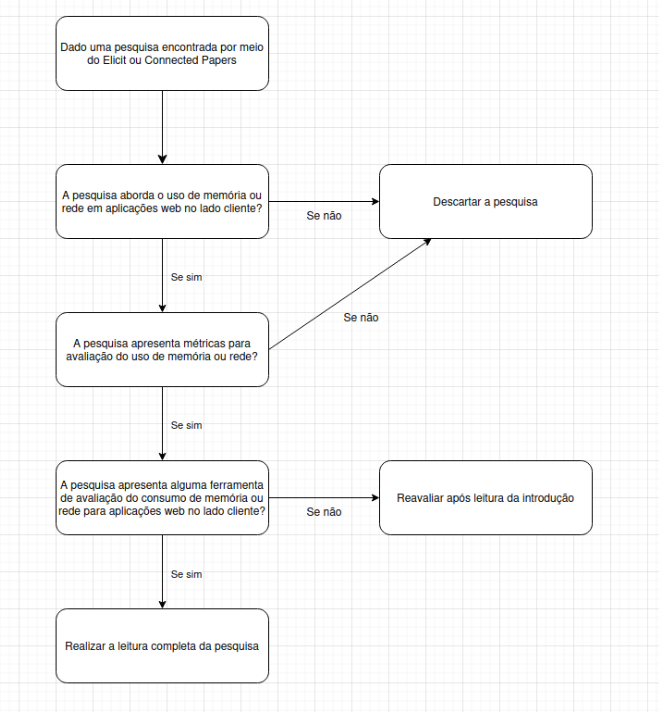
\includegraphics[width=0.6\textwidth]{figures/paper-decision-tree.png}
	\caption{Critérios utilizados para seleção de trabalhos para leitura.}
	\label{fig:fluxo-leitura}
\end{figure}

\begin{table}[!ht]
	\centering
	\caption{Total de trabalhos encontrados.}
	\begin{tabular}{l  c L{1.5cm} R{1.5cm}}
		\toprule
		\textbf{Ferramenta} & \textbf{Trabalhos Encontrados} \\
		\midrule
		Elicit  &  280  \\
		Connected Papers  &  120  \\
		\midrule
		Total  &  400  \\
		\bottomrule
	\end{tabular}
	\label{tab:trabalhos-encontrados}
\end{table}

\chapter{Trabalhos Relacionados}
\label{sec:trabalhos_relacionados}
	\label{sec:trab_relacionados}

	% \item \textbf{Paper 1}: Summary of the first paper goes here. This paragraph provides a concise overview of the paper's objectives, methodology, and key findings.
	\section{Ferramentas Para Medição no Lado do Cliente}
	Utilizando os métodos descritos na seção anterior do trabalho, conseguimos levantar um panorama geral dos frameworks e soluções existentes e propostos à academia, assim como classifica-los utilizando alguns parâmetros, afim de entender se a nossa proposta se demonstra complementar ao estado da arte. 
	Os critérios da classificação são: 


	\begin{table}[!ht]
		\centering
		\caption{Strings de busca utilizadas na ferramenta Connected Papers.}
		\begin{tabular}{c c L{1.5cm} R{1.5cm}}
			\toprule
			\textbf{Critério} & \textbf{Descrição}\\
			\midrule
			Arquitetura Simples & Se a arquitetura da ferramenta é de fácil entendimento\\
			Flexibilidade&Se a ferramenta se adapta em diversos contextos de medição\\
			Curva de Apredizado&Se a ferramenta possui uma curva de aprendizado rápida\\
			Multiplataforma&Se a ferramenta suporta o uso em diversas plataformas\\
			Persistência&Se a ferramente persiste dados para análise futura\\
			\bottomrule
		\end{tabular}
		\label{tab:string-busca-connected-papers}
	\end{table}


	\par Dessa forma, a classificação dos trabalhos selecionados se encontra na tabela abaixo:

		\begin{table}[ht]
			\scriptsize
			\caption{Classificação das Ferramentas Encontradas} % title of Table
			\centering % used for centering table
			\begin{tabular}{c c c c c c} % centered columns (4 columns)
			\hline\hline %inserts double horizontal lines
			\textbf{Plataforma} & \textbf{Arquitetura Simples} & \textbf{Flexibilidade} & \textbf{Curva de Aprendizado} & \textbf{Multiplataforma} & \textbf{Persistência} \\[0.5ex]

			%heading
			\hline % inserts single horizontal line
			MemInsight & sim & não & sim & sim & não \\
			WePR & não & não & não & sim & sim \\
			Gember & sim & não & sim & não & sim \\
			Mobilyzer & sim & não & não & não & sim \\
			\hline %inserts single line
			\end{tabular}
			\label{table:nonlin} % is used to refer this table in the text
		\end{table}
	

		\subsection{MemInsight}
		\par No contexto de medição de memória, temos a MemInsight \citep{Jensen2015MemInsight}. Essa ferramenta roda de forma independente sobre uma engine Javascript, não precisando de um browser para executar, e faz a análise do consumo de memória através de um conjunto de traces, dados estruturados que tornam possível remontar o ciclo de vida dos objetos em memória, e que permitem a análise de desperdício de recursos durante a execução do programa. 
		\par Analisando a ferramenta, foi observado que ela só trabalha com medição de métricas de memória, não permitindo generalizar consultas de outros tipos, por isso classificamos como não flexível com relação as métricas. Além disso, por ser uma ferramenta orientada ao “debug” de aplicações, não realiza nativamente a persistência e organização desses dados.
		

		\subsection{WePR}
		\par \citep{Asrese2019MeasuringWL} também propôs uma feramenta para medição client-side, porém agora com o enfoque em medir métricas de \acr{QoS}, nomeada WePR. No trabalho, ele apresenta um panorama da evolução da web, especialmente de como a latência se desenvolveu nos websites, e sustenta a necessidade desse tipo de medição como forma de melhorar a experiência do usuário, que indicam ser um fator determinante no abandono ou sucesso de um website. A ferramenta foi testada utilizando grandes websites como Google, Youtube e Facebook. 
		\par A arquitetura da ferramenta é distribuida, e consiste basicamente de um coletor, um servidor que fornece os elementos das páginas para medição, múltiplos servidores de renderização gerenciados por um balanceador (loadbalancer), e um servidor que cuida da persistência dos dados. Dessa forma, o coletor inicialmente pede ao servidor os URL’s dos elementos a serem medidos, e após obter essa resposta, faz o download desses elementos e captura métricas. Posteriormente, envia esses dados medidos e os elementos baixados para o loadbalancer, e por fim algum dos servidores de renderização envia os dados para persistência.
		\par O enfoque da ferramenta é a medição de performance de websites, dessa forma sua arquitetura e usabilidade não foram construídas de forma simples de extender, tornando dificil a utilização da ferramenta em outros contextos. Além disso, não temos a possibilidade de customizar as métricas, o que torna pouco flexível quando se trata de outras medições, como métricas de performance por exemplo.
		
		\subsection{Gember}
		\par \citep{Gember2012Obtaining} também traz um estudo sobre medição client-side, porém dessa vez em clientes móveis, utilizando dados de um provedor de internet e também de experimentos controlados. Esse tipo de medição é muito útil para provedores de internet e desenvolvedores, que precisam entender como suas aplicações performam interagindo com a rede móvel de internet.
		\par Foi desenvolvido no trabalho um protótipo para Android de um medidor de performance para analisar somente quando o dispositivo está ativo, e que é integrado ao app como uma biblioteca. A arquitetura consiste basicamente de um controlador central (servidor), e múltiplos clientes (aparelhos) com o código rodando em seus celulares. Dessa forma, o pesquisador faz uma requisição para esse controlador, e ele coordena a coleta do que foi solicitado nos aparelhos, salvando os resultados no servidor.
		\par O serviço inicialmente coleta latência, throughput, streaming e o tempo de carregamento de páginas web, mas é extensível para outras métricas de rede. A limitação aqui é a utilização no cliente, somente no ambiente mobile Android, tornando pouco flexível a utilização dessa ferramenta entre diferentes plataformas, e também a coleta somente de informações de rede.

		\subsection{Mobilyzer}
		\par Ainda no contexto de medição de rede, se encontra o Mobilyzer \citep{Nikravesh2015Mobilyzer}, uma plataforma aberta para medição de rede em dispositívos móveis. Essa plataforma foi criada com o objetivo de prover uma solução escalável, eficiente e controlável, que fosse possível de ser incorporada tanto a apps em desenvolvimento, quanto em apps que já estão desenvolvidos, para suportar pesquisas e testes em medição de rede. 
		\par Ela funciona utilizando alguns componentes básicos, sendo eles: 
		\begin{enumerate}
			\item Uma biblioteca Android, que é integrada aos aplicativos para coletar as informações e enviar ao servidor. Ela é incorporada direto no código fonte.
			\item Um componente chamado gerenciador de memória, no qual o pesquisador pode inserir medições de forma customizada e mais eficiente. Ele também realiza o scheduling das medições, e também cordena e monitora os dispositivos para que não tenha sobrecarga em nenhum aparelho ou rede medida. 
			\item Um servidor na núvem, que fica responsável por coletar, analisar aplicando regras e publicar os dados coletados dos dispositivos. Essa arquitetura centralizada simplifica o compartilhamento de dados entre essas etapas, podendo integrar outras ferramentas de analise de dados com a base das coletas.

		\end{enumerate}
		\par Uma dificuldade no uso do Mobilyzer em pesquisas é que essa plataforma também se restringe ao ambiente mobile, e apenas na plataforma Android. Isso diminui bastante possibilidades de medição em pesquisas multiplataforma. Além disso, não temos muita flexibilidade com relação as métricas, sendo em sua maior parte métricas de rede.

		\subsection{FadeCow}
		\par Após o descrito, podemos posicionar o FadeCow com relação aos critérios que estabelecemos no começo dessa secção. Temos um modelo de arquitetura simples, a possibilidade de expandir e construir métricas diversas, uma curva de aprendizado suave, a compatibilidade com múltiplas plataformas, pois a coleta das métricas ocorre no browser, e também a persistência desses dados para futura análise.
		\par Assim, a tabela teria a seguinte configuração após a adição do FadeCow:

		\begin{table}[ht]
			\scriptsize
			\caption{Classificação das Ferramentas Encontradas Após Adição do FadeCow} % title of Table
			\centering % used for centering table
			\begin{tabular}{c c c c c c} % centered columns (4 columns)
			\hline\hline %inserts double horizontal lines
			\textbf{Plataforma} & \textbf{Arquitetura Simples} & \textbf{Flexibilidade} & \textbf{Curva de Aprendizado} & \textbf{Multiplataforma} & \textbf{Persistência} \\[0.5ex]

			%heading
			\hline % inserts single horizontal line
			MemInsight & sim & não & sim & sim & não \\
			WePR & não & não & não & sim & sim \\
			Gember & sim & não & sim & não & sim \\
			Mobilyzer & sim & não & não & não & sim \\
			FadeCow & sim & sim & sim & sim & sim \\
			\hline %inserts single line
			\end{tabular}
			\label{table:nonlin} % is used to refer this table in the text
		\end{table}

\chapter{Método} 
\label{cap:metodologia}

\section{Exemplo conceitual: Comparando o desempenho entre os formatos de arquivo JSON e CSV}

Imagine que você seja um pesquisador ou um desenvolvedor que decidiu utilizar a nossa ferramenta para sanar uma dúvida que encontrou ao desenvolver sua pesquisa:
O que possui melhor desempenho em um grande conjunto de dados? Transferir usando um arquivo CSV ou um arquivo JSON? A nossa ferramenta poderia ajudar.

Modelando o problema, o Projeto seria a sua aplicação, que seria composto por Tarefas, ou seja, a Tarefa é o que você realiza na sua aplicação e deseja realizar medições. Porém, podemos ter Tarefas simples, como no caso de uma medição única do tempo de download do arquivo, ou Tarefas Compostas, que poderia ser um pipeline completo de download e consulta utilizando um dos formatos de arquivo (realizar o download do arquivo, abrir no registro x dentro do arquivo, imprimir a informação). Ou seja, existe uma grande flexibilidade na elaboração de Tarefas.

A análise seria um conjunto de métricas. No nosso exemplo, algumas métricas possíveis são:

\begin{itemize}
	\item Tempo gasto.
	\item Largura de banda.
	\item Tamanho do arquivo.
	\item Informações do ambiente de execução.
	\item Gasto de memória.
\end{itemize}

Essas métricas, quando agrupadas, dão forma a uma análise, que representa uma medição utilizando um dos métodos a serem testados. No nosso exemplo, teríamos ao final do experimento duas análises: uma referente as medições acima utilizando o método CSV e outra utilizando o método JSON.

\section{Diagrama conceitual}

Na elaboração de qualquer projeto de software, a construção de um bom esquema conceitual é extremamente importante e fundamental para o sucesso do desenvolvimento. Na nossa ferramenta, possuímos algumas entidades principais. São elas:

\begin{figure}[!ht]
	\centering
	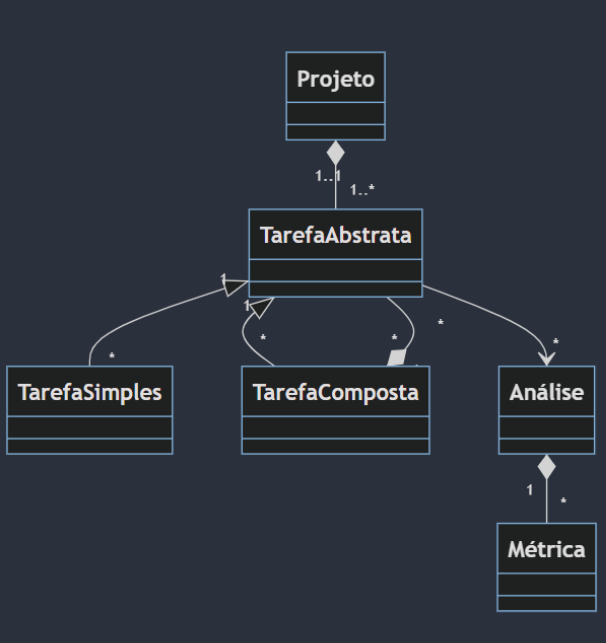
\includegraphics[width=0.6\textwidth]{figures/diagrama-conceitual.png}
	\caption{Diagrama conceitual.}
	\label{fig:diag-conceitual}
\end{figure}

\begin{description}
	\item[Projeto:] Aplicação na qual o pesquisador está avaliando suas provas de conceito. É composto de uma lista de tarefas associadas, que constituem as ações que são executadas na aplicação e que desejam ser medidas pelo pesquisador/desenvolvedor. A cardinalidade da relação entre o Projeto e as Tarefas é de 1 para muitos, pois o Projeto deve ter pelo menos uma ou muitas Tarefas associadas a ele. 
	Ex: Projeto de construção de um transferidor de dados. Tarefas: fazer o download do arquivo, realizar a execução de um pipeline de consulta.
	
	\item[Tarefa Abstrata:] 
	Alguma ação executada no projeto com início, meio e fim. É representada por uma entidade abstrata, pois representa conceitualmente o que precisa ser executado no projeto. Pode ser descrita também como um roteiro de um processo ou procedimento sob avaliação. Essas ações podem ser fornecidas pelo pesquisador, ou pode ser parametrizada inicialmente pela ferramenta.

	\item[Tarefa Composta:] 
	Representa um conjunto de tarefas. Ex: Realização de um pipeline de consulta no arquivo (Tarefas agregadas: Realizar o download do arquivo, abrir o arquivo na linha X, realizar leitura).
	Utilizamos nessa entidade o padrão de software Composite, que nos permite representar facilmente um agrupamento de uma entidade. Nesse caso, a entidade folha seria uma Tarefa Simples, e o agrupamento a Tarefa Composta. Realizamos essa escolha pois simplifica a execução de múltiplas tarefas ao mesmo tempo, no caso de ser executado um pipeline grande de tarefas.

	\item[Análise:] 
	Um conjunto de métricas coletadas da execução de uma tarefa utilizando um método. Essas métricas correspondem aos dados desejados pelo pesquisador, e uma análise deve possuir uma ou mais métricas.
	Dessa forma, a saída das execuções das tarefas é uma análise, composta pelas métricas desejadas pelo pesquisador, e que se relaciona a Tarefa Abstrata. Uma Tarefa Abstrata pode estar relacionada a uma ou mais análises, e as análises podem estar relacionadas a uma ou mais tarefas, visto que é um agrupamento de métricas. Diferentes métodos gerarão diferentes análises, cada uma com as suas métricas.
	Ex: Uma Análise dos métodos de transferência de dados seria composta por: um cojunto de métricas, qual tarefa ela representa, e qual método ela está representando. Nesse caso teríamos duas análises, uma com o método JSON e uma com o método CSV.

	\item[Métrica:] 
	Uma medida quantitativa de algum recurso computacional do cliente. Ou seja, a unidade mais granular do sistema. Pode ser fornecida pela ferramenta ou inserida pelo pesquisador. Ex: O conjunto de métricas da Análise dos métodos de transferência de dados seria composto por: velocidade de transferência, tamanho do arquivo, tempo total de transferência, taxa de compressão do arquivo, entre outras.

\end{description}


\section{Diagrama de Classes}

Após a elaboração do diagrama conceitual, foi elaborado o Diagrama de Classes à seguir que dará base a implementação do sistema: 

O diagrama começa com a entidade Project, que representa um projeto, e que possui um método que executa todas as tarefas associadas a ele.
Além disso, um detalhe importante nessa entidade é o relacionamento com ExecutionProfile, que seria qual cliente está executando aquele projeto. Temos também que o Project pode possuir um ou mais IPersister, que é o método abstrato que representa os repositórios que realizarão as interações com as bases de dados. Em IPersister, podemos ter diversas instâncias.
No diagrama foi criada somente a SheetsonPersister, que será a nossa escolha inicial para base de dados.

Em seguida, vemos a classe abstrata Task, que representa as tarefas abstratas.
Ela possui o método público run(), que será como essa tarefa será executada, e os métodos privados execute(), preTaskJob() e postTaskJob(), que serão implementados pelas classes concretas.
Eles representam, respectivamente, a execução detalhada da tarefa, um conjunto de operações a serem realizadas antes da execução, e um conjunto de atividades a serem realizadas depois da execução da tarefa.

Após isso, temos a classe abstrata Metric, ou Métrica.
Nela temos os métodos públicos collect() e get(), que serão as interações externas com as métricas.
Temos também o método privado preProcessing(), que serve para realizar, se necessário, algum pré-processamento antes da coleta da métrica.
Temos dois exemplos de implementações concretas dessa classe no diagrama, são eles:
ProcessMemoryMetric e DeltaTimeMetric. O exemplo DeltaTimeMetric possui uma necessidade de pré-processamento, já que a variação de tempo é calculada com base em dois parâmetros diferentes, o que justifica a implementação desse método.


\begin{figure}[!ht]
	\centering
	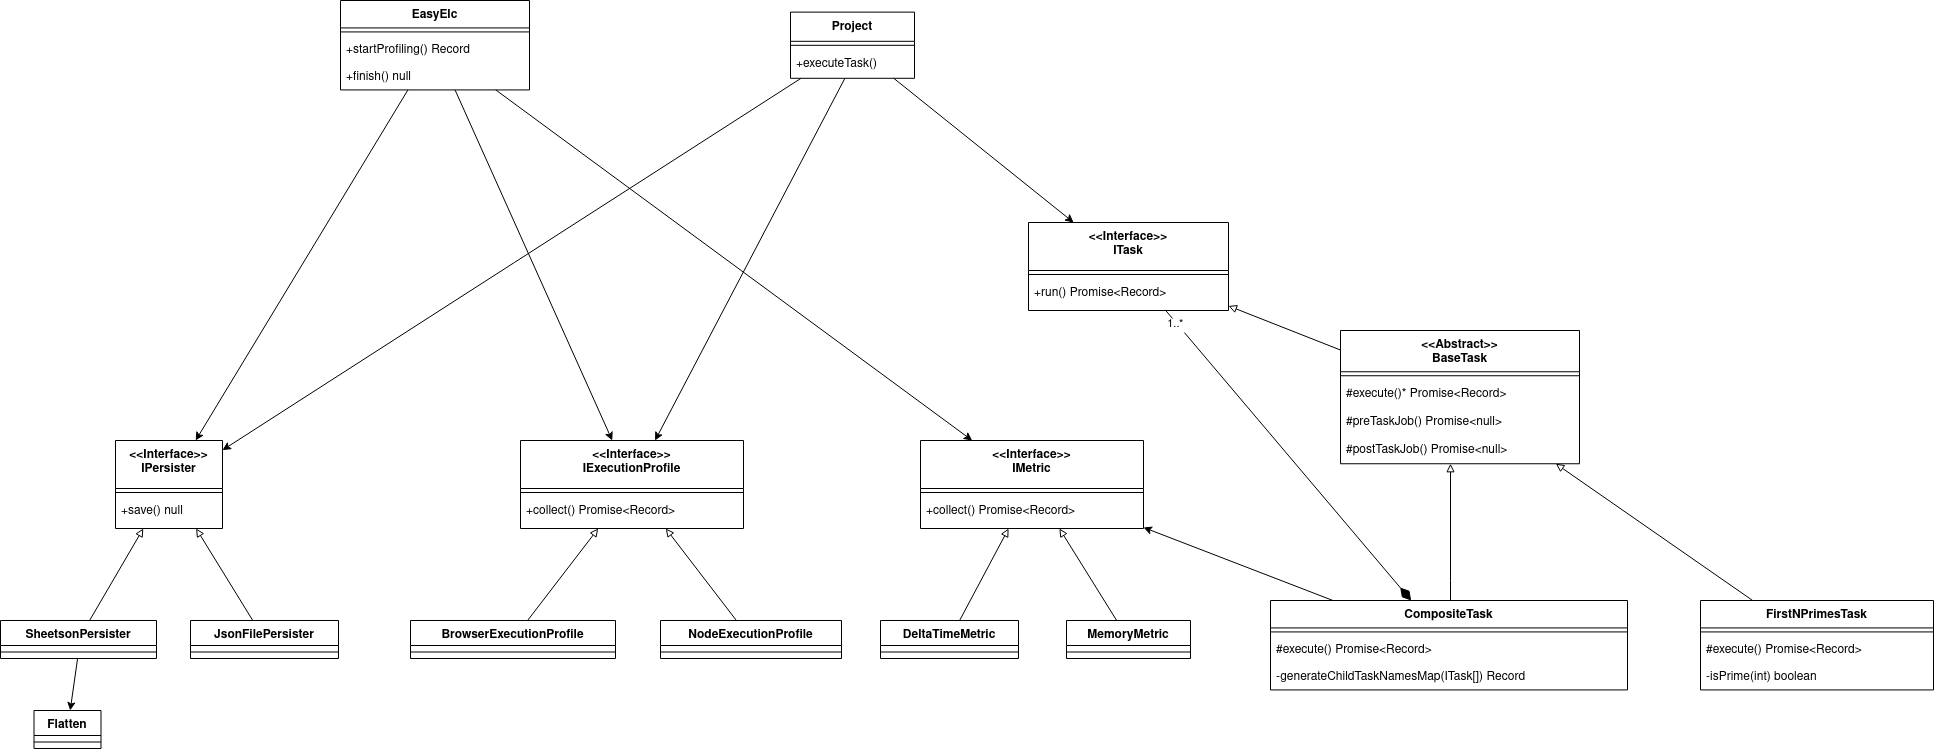
\includegraphics[width=0.6\textwidth]{figures/diagrama-classes.png}
	\caption{Diagrama classes.}
	\label{fig:diag-classes}
\end{figure}


\section{Arquitetura}

Na utilização da aplicação, o pesquisador deve ser capaz de inserir suas métricas, suas análises, e chamar no código dele os métodos de coleta. Dessa forma, precisamos construir um ambiente no qual ele consiga realizar essas tarefas. Isso pode ser feito de diferentes formas, uma delas chamamos de abordagem tradicional, e a outra que propomos é utilizando a ferramenta Sheetson.

\subsection{Abordagem tradicional}

Nessa abordagem seria realizada a implementação de dois componentes principais: 

\begin{description}
	\item[Biblioteca Javascript:] Esse componente diz respeito a biblioteca que o pesquisador inserirá no código da sua aplicação, inserindo nela as métricas desejadas para medição.

	\item[Backend na núvem:] Esse componente receberia as requisições enviadas pela aplicação e condensaria em um banco de dados qualquer essas medições. Após isso, seria necessário o desenvolvimento de um front-end, para o pesquisador conseguir baixar esses arquivos.
\end{description}

Essa abordagem seria a mais comum, dado que possui similaridades com grande parte das aplicações que vemos hoje. Porém, essa implementação deixaria a aplicação com uma alta complexidade de uso, e além disso, não seria escalável, pois o backend precisa de adaptações para lidar com, por exemplo, múltiplos bancos de dados.
Nesse contexto, encontramos uma solução que se demonstrou interessante para o nosso problema.

\subsection{Sheetson}

O Sheetson é uma ferramenta gratuita, a qual torna possível a inserção e interação com uma planilha do Google Docs via API. Então a solução baseada nessa ferramenta seria:

\begin{description}
	\item[Biblioteca Javascript:] Esse componente diz respeito a biblioteca que o pesquisador inserirá no código da sua aplicação, inserindo nela as métricas desejadas para medição.
	
	\item[Sheetson:] O Sheetson receberia os dados enviados do cliente, e inseriria em uma tabela CSV, para download futuro.

\end{description}

Essa abordagem possui diversas vantagens, como poder isolar no desenvolvimento da biblioteca a classe que controlará a persistência dos dados, e implementar inicialmente utilizando o sheetson. Se quisermos posteriormente implementar a primeira abordagem e substituir por chamadas a um backend real, com qualquer base de dados que seja, seria necessário somente substituir essa implementação, porém hoje ganharíamos um tempo grande no desenvolvimento do projeto.

Além disso, o pesquisador poderia utilizar sua própria conta do Google para realizar suas pesquisas, eliminando a necessidade de contratar provedores de cloud ou de fazer deploy de alguma aplicação. Isso gera uma redução grande na complexidade do uso do projeto.


\chapter{Estado Atual do Trabalho}
\label{cap:estado_atual}

Com a definição do framework e seu escopo em mãos, realizamos a pesquisa a qual origina o capítulo \ref{cap:fund_teorica}.
Tendo como objetivo, confirmar se há espaço dentro do ecossistema das ferramentas de análise de desempenho e recursos computacionais para o que estamos propondo.
Como dentre as ferramentas encontradas não havia uma voltada para que um desenvolvedor seja capaz de avaliar provas de conceito de modo customizável em diversos tipos de configurações do lado do cliente, concluímos que há espaço para a proposta do nosso framework.

Após isso, o próximo passo foi a definição dos conceitos do framework.
Para tanto, elaboramos o diagrama conceitual o qual tem o papel de definir como os objetivos do framework devem ser alcançados e planejar as principais características da arquitetura do projeto.
Por exemplo, nessa etapa foi onde definimos que o padrão de projeto Composite seria utilizado, com o objetivo de permitir que uma prova de conceito seja dividida em etapas as quais possuem suas próprias métricas.
Deste modo, fica a critério do usuário se sua abordagem trata as provas de conceito como um bloco único ou como um conjunto de etapas, o que pode permitir diagnósticos de desempenho mais precisos.

O terceiro passo foi voltado para a arquitetura do projeto.
Onde elaboramos o diagrama de classes e avaliamos os principais aspectos práticos de seu desenvolvimento.
Dentre eles, o ponto de maior destaque foi como realizar a captura das métricas de execuções realizadas por voluntários.
Pois, uma abordagem tradicional ao problema envolveria o desenvolvimento de uma \acr{API} para nos permitir receber e disponibilizar a consulta dos dados.
Entretanto, disponibilizar os dados dos usuários do framework na Internet tornaria necessário também criar uma camada de autorização, expandindo ainda mais o escopo de desenvolvimento.
A solução encontrada para o problema foi a utilização do programa de planilhas online Google Sheets, onde ao invés da execução do framework enviar as métricas para uma \acr{API} nossa, ela envia para uma planilha do próprio usuário.
Deste modo, não há a necessidade do desenvolvimento de \acr{API}, pois, utilizariamos uma do Google Sheets e o controle de acesso aos dados também fica sob responsabilidade deles.

A última etapa atual está sendo o desenvolvimento de uma prova de conceito do próprio framework.
Para tanto, optamos por desenvolver utilizando a linguagem de programação TypeScript, a fim de exercitar as classes e relações planejadas durante a criação dos diagramas.
Nela estamos utilizando objetos mock, a fim de simular comportamentos do ambiente como consumo de memória e tempo gasto na execução de tarefas.
Além de simular como um usuário do framework aplicaria a estrutura de árvore de tarefas em suas provas de conceito.
Durante essa etapa também encontramos algumas limitações do conceitos como a inaplicabilidade do conceito de análise como uma avaliação independente de tarefas, pois, seria necessário restringir a liberdade na obtenção de métricas.

O desenvolvimento do framework e produção textual estão sendo realizados em paralelo.
A fundamentação teórica, capítulo \ref{cap:fund_teorica}, se encontra em fase de desenvolvimento e tem conclusão prevista para outubro de 2023.
A descrição do framework, capítulo \ref{cap:metodologia}, será descrita de forma mais precisa e detalhada até janeiro de 2024, junto com um exemplo de sua utilização.
A defesa da dissertação está prevista para janeiro de 2024. O cronograma indicado na tabela \ref{tab:cronograma} prevê as etapas abordadas neste trabalho.
A tabela indica os meses de previsão de conclusão de cada uma das etapas.

\begin{table}[!ht]
	\centering
	\caption{Cronograma de desenvolvimento da dissertação}
	\begin{tabular}{l  c  c  c  c  c  c L{1.5cm} R{1.5cm}}
		\toprule
		\textbf{Atividade} & \textbf{fev-mar} & \textbf{abr-mai} & \textbf{jun-jul} & \textbf{ago-set} & \textbf{out-nov} & \textbf{dez-jan} \\
		\midrule
		Planejamento e Escopo  &  X  &    &    &    &    &    \\
		Fundamentação Teórica  &  X  &  X  &    &    &    &    \\
		Arquitetura  &    &  X  &  X  &    &    &    \\
		Prova de Conceito  &    &    &  X  &  X  &    &    \\
		Desenvolvimento  &    &    &    &  X  &  X  &    \\
		Exemplo de Uso  &    &    &    &    &  X  &  X  \\
		Defesa  &    &    &    &    &    &  X  \\
		\bottomrule
	\end{tabular}
	\label{tab:cronograma}
\end{table}

\label{bibpage}
\renewcommand\bibname{Referências}
\addcontentsline{toc}{section}{Referências}
\bibliography{references}
%\bibliographystyle{plainnat}
\bibliographystyle{apalike}
\label{bibfinalpage}

\label{lastpage}

\section{Codigo da prova de conceito}

\subsection{Project.ts}
\lstinputlisting[language=TypeScript]{./mock/Project.ts}

\subsection{Index.ts}
\lstinputlisting[language=TypeScript]{./mock/Index.ts}

\subsection{Tasks/Task.ts}
\lstinputlisting[language=TypeScript]{./mock/Tasks/Task.ts}

\subsection{Tasks/MockTask.ts}
\lstinputlisting[language=TypeScript]{./mock/Tasks/MockTask.ts}

\subsection{Tasks/CompositeTask.ts}
\lstinputlisting[language=TypeScript]{./mock/Tasks/CompositeTask.ts}

\subsection{Tasks/SimpleTask.ts}
\lstinputlisting[language=TypeScript]{./mock/Tasks/SimpleTask.ts}

\subsection{Persister/IPersister.ts}
\lstinputlisting[language=TypeScript]{./mock/Persister/IPersister.ts}

\subsection{Persister/SheetsonPersister.ts}
\lstinputlisting[language=TypeScript]{./mock/Persister/SheetsonPersister.ts}

\subsection{Helpers/Helpers.ts}
\lstinputlisting[language=TypeScript]{./mock/Helpers/Helpers.ts}

\subsection{Helpers/MockResource.ts}
\lstinputlisting[language=TypeScript]{./mock/Helpers/MockResource.ts}

\subsection{Metrics/AbstractMetric.ts}
\lstinputlisting[language=TypeScript]{./mock/Metrics/AbstractMetric.ts}

\subsection{Metrics/GetDeltaTime.ts}
\lstinputlisting[language=TypeScript]{./mock/Metrics/GetDeltaTime.ts}

\subsection{Metrics/GetResourceUsage.ts}
\lstinputlisting[language=TypeScript]{./mock/Metrics/GetResourceUsage.ts}

\end{document}